\documentclass{article}
\usepackage[margin=1in]{geometry}
%\VignetteIndexEntry{How to use RSGHB}

\usepackage{url}
\makeatletter
\def\url@leostyle{%
  \@ifundefined{selectfont}{\def\UrlFont{\sf}}{\def\UrlFont{\small\ttfamily}}}
\makeatother
\urlstyle{leo}

\usepackage{Sweave}
\begin{document}

\title{How to use RSGHB}
\author{Jeffrey Dumont}
\date{6 April 2013}
\maketitle
\abstract{This vignette describes the process for specifying, estimating and analyzing the output of a choice model with RSGHB. The document is structured into two case studies using different model structures. The synthetic choice data used in this document (as well as number of other examples using different model structures) can be downloaded from RSGHB github page - \url{https://github.com/jeffdumont/RSGHB}}

\begin{center}
\line(1,0){400}
\end{center}

\section*{RSGHB modeling file structure}

The typical RSGHB model file has the following 4 main sections. We will walk through each of these 4 sections in the examples that follow.

\begin{enumerate}
     \item Setup and data preparation
     \item Setting the controls for model estimation
     \item Defining the likelihood function
     \item Calling the doHB function to start the estimation process
\end{enumerate}

\section*{EXAMPLE 1: MNL Model with Fixed Parameters}

In this section, the code for estimating a multinomial logit model with fixed (non-random) parameters is explained. In this example, synthetic respondents were presented with a choice between two travel alternatives - one that is toll free but slower and one that was priced but faster. Each respondent was presented with a panel of 8 choice tasks.

\subsection*{Setup and Data Preparation}

\begin{Schunk}
\begin{Sinput}
> library(RSGHB)
> # load example data
> data(choicedata)
> # We typically work with one one row per choice observations. This isn't necessary however but it does lend it self to faster computation of the choice likelihoods
> head(choicedata)
\end{Sinput}
\begin{Soutput}
    ID thecount tt1 tt2 toll2 asc1 Choice
1 8738        1  60  51  1.25    1      1
2 8738        2  60  51  0.75    1      1
3 8738        3  63  59  0.50    1      2
4 8738        4  60  54  0.75    1      1
5 8738        5  60  54  0.50    1      2
6 8738        6  63  54  0.75    1      1
\end{Soutput}
\begin{Sinput}
> # We can then specify any variables from the choicedata data.frame that you'd like to use in the
> # utility equations in the likelihood function below. These can be any variables within the data or transformations of those variables. This example comes from transport so each alternative is defined by travel times and toll costs.
> TT1     <- choicedata$tt1
> TT2     <- choicedata$tt2
> TOLL2   <- choicedata$toll2
> # Here we specify the choice vectors. Note in this example there are only two alternatives. Also, dummying coding the choice vector is not necessary but allows for easier coding of the likelihood.
> choice1    <- (choicedata$Choice==1)
> choice2    <- (choicedata$Choice==2)
> # Frequency of choice for the first alternative
> table(choice1)
\end{Sinput}
\begin{Soutput}
choice1
FALSE  TRUE 
 3560  6682 
\end{Soutput}
\begin{Sinput}
> # Frequency of choice for the second alternative.
> table(choice2)
\end{Sinput}
\begin{Soutput}
choice2
FALSE  TRUE 
 6682  3560 
\end{Soutput}
\begin{Sinput}
> 
\end{Sinput}
\end{Schunk}

\subsection*{Controling the Estimation Process}

There are number of options for controling the estimation process. Please see the help file for doHB or the final section of this document for more details. Note that a number of controls have default values and do not need to be directly specified if the default is acceptable.

\begin{Schunk}
\begin{Sinput}
> # ------------------
> # ESTIMATION CONTROL
> # ------------------
> 
> # Setting control list for estimation (see ?doHB for more estimation options)
> 
> # modelname is used for naming the output files
> modelname <- "MNL"          
> # gVarNamesFixed contains the names for the fixed (non-random) variables in your model. This will be used in output and also when displaying iteration detail to the screen.
> gVarNamesFixed <- c("ASC1","BTime","BCost")
> # FC contains the starting values for the fixed coefficients.
> FC <- c(0,0,0)                 
> # ITERATION SETTINGS
> 
> # gNCREP contains the number of iterations to use prior to convergence
> gNCREP    <- 30000
> # gNEREP contains the number of iterations to keep for averaging after convergence has been reached
> gNEREP    <- 20000 	       
> # gNSKIP contains the number of iterations to do in between retaining draws for averaging
> gNSKIP    <- 1		       
> # gINFOSKIP controls how frequently to print info about the iteration process
> gINFOSKIP <- 250           
> # To simplify the doHB functional call, we put all of the control parameters into a single list that can be passed directly to doHB.
> control <- list(
+      modelname=modelname,
+      gVarNamesFixed=gVarNamesFixed,
+      FC=FC,
+      gNCREP=gNCREP,
+      gNEREP=gNEREP,
+      gNSKIP=gNSKIP,
+      gINFOSKIP=gINFOSKIP
+ )
> 
\end{Sinput}
\end{Schunk}

\subsection*{Writing the likelihood function}

RSGHB is expecting the user-specificed likelihood function to take the parameters \emph{fc} and \emph{b} (even if they are not used within the function calculate the likelihood). The \emph{fc} parameter is a vector of fixed coefficients (they do not vary across individuals in your data). The \emph{b} parameter is a matrix of individual coefficients which are generated from the random coefficients in the model. In this example, we only focus on the \emph{fc} vector.

It is important to note that the computation of the likelihood is the most computational taxing part of the estimation process. So coding the likelihood efficiently is essential to reduce run time of the model.


\begin{Schunk}
\begin{Sinput}
> # ------------------
> # likelihood
> # ------------------
> 
> likelihood <- function(fc,b)
+ {
+ 
+   # defining the parameters          
+ 
+   # using cc var to index the fc vector simplifies the addition/subtraction of new parameters     
+   cc <- 1
+   ASC1   <- fc[cc];cc <- cc+1
+   Btime  <- fc[cc];cc <- cc+1
+   Btoll  <- fc[cc];cc <- cc+1  
+ 
+   # utility functions
+   v1 <- ASC1       + Btime * TT1                   
+   v2 <-              Btime * TT2 + Btoll * TOLL2   
+  
+   # mnl probability statement
+   p  <- (exp(v1)*choice1 + exp(v2)*choice2) / (exp(v1) + exp(v2))
+ 	
+   return(p)
+ }
\end{Sinput}
\end{Schunk}

\subsection*{Estimating the model}

To start the model estimation process, the analyst needs to call the \emph{doHB} function passing in the \emph{likelihood} function, the \emph{choicedata} data.frame and the \emph{control} list. 

\begin{verbatim}
doHB(likelihood, choicedata, control)
\end{verbatim}

RSGHB will first perform a series of diagnostics on your model to catch common errors in model setup. In addition, it will provide you with some basice summary statistics on your choice data and model. Before estimation begins, RSGHB will present you with a confirmation prompt allowing you to cancel the model estimation.

\begin{figure}
\caption{Plotting of the Markov Chains during estimation}
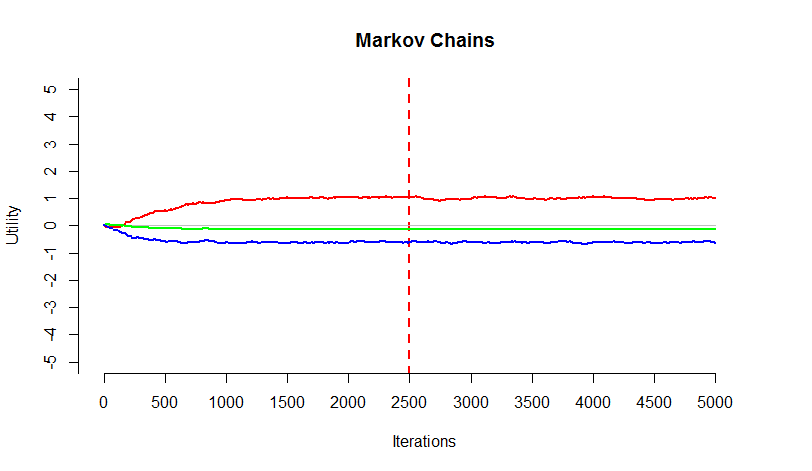
\includegraphics[scale=0.50]{MNL_markovChains.png}
\label{MarkovChain}
\end{figure}

During the estimation, current estimates of the markov chains will be plotted to the screen. This plot is updated based on the control parameter \emph{gINFOSKIP} (see figure \ref{MarkovChain}). In addition, it will provide numerical iteration details in the R Console.



\subsection*{Evaluating the output}

There are two main output files for this particular model - \emph{log} file and the \emph{\_F} file. RSGHB comes with some basic tools for plotting the contents of these files.

The \emph{.log} file contains some statistics that can be used to understand if model convergence has been reached. Because this model contains only fixed coefficents, the log file contains just the root likelihood (RLH) and log-likelihood at each iteration defined by \emph{gINFOSKIP} - see figure \ref{logfile1}.

\begin{figure}
\caption{Plotting of the Log file}
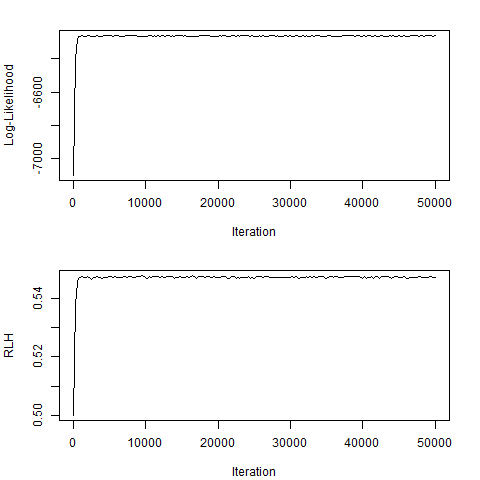
\includegraphics[scale=0.50]{MNL_logPlot1.png}
\label{logfile1}
\end{figure}

The \emph{\_F} file contains the set of fixed (non-random) coefficients for each iteration after convergence of the markov chain.

\begin{Schunk}
\begin{Sinput}
> data(Example1_F)
> head(Example1_F)
\end{Sinput}
\begin{Soutput}
  iteration     ASC1      BTime      BCost
1         1 1.030406 -0.1460260 -0.6586186
2         2 1.030406 -0.1460260 -0.6586186
3         3 1.030406 -0.1460260 -0.6586186
4         4 1.030406 -0.1460260 -0.6586186
5         5 1.030406 -0.1460260 -0.6586186
6         6 1.027050 -0.1450802 -0.6579254
\end{Soutput}
\begin{Sinput}
> 
\end{Sinput}
\end{Schunk}



\section*{EXAMPLE 2: MNL Model with Random Coefficients}

In this section, we expand on the model estimated in EXAMPLE 1 by allowing the coefficients to vary across the individuals in our dataset. This type of model is referred to by many names - Random Coefficients Logit, Random Parameters Logit or Mixed Logit. 

\subsection*{Setup and Data Preparation}

The setup and data preparation are very similar to the first model.

\begin{Schunk}
\begin{Sinput}
> library(RSGHB)
> # load example data
> data(choicedata)
> # We typically work with one one row per choice observations. This isn't necessary however but it does lend it self to faster computation of the choice likelihoods
> head(choicedata)
\end{Sinput}
\begin{Soutput}
    ID thecount tt1 tt2 toll2 asc1 Choice
1 8738        1  60  51  1.25    1      1
2 8738        2  60  51  0.75    1      1
3 8738        3  63  59  0.50    1      2
4 8738        4  60  54  0.75    1      1
5 8738        5  60  54  0.50    1      2
6 8738        6  63  54  0.75    1      1
\end{Soutput}
\begin{Sinput}
> # We can then specify any variables from the choicedata data.frame that you'd like to use in the
> # utility equations in the likelihood function below. These can be any variables within the data or transformations of those variables. This example comes from transport so each alternative is defined by travel times and toll costs.
> TT1     <- choicedata$tt1
> TT2     <- choicedata$tt2
> TOLL2   <- choicedata$toll2
> # Here we specify the choice vectors. Note in this example there are only two examples. Also, dummying coding the choice vector is not necessary but allows for easier coding of the likelihood.
> choice1    <- (choicedata$Choice==1)
> choice2    <- (choicedata$Choice==2)
> # Frequency of choice for the first alternative
> table(choice1)
\end{Sinput}
\begin{Soutput}
choice1
FALSE  TRUE 
 3560  6682 
\end{Soutput}
\begin{Sinput}
> # Frequency of choice for the second alternative.
> table(choice2)
\end{Sinput}
\begin{Soutput}
choice2
FALSE  TRUE 
 6682  3560 
\end{Soutput}
\begin{Sinput}
> 
> 
\end{Sinput}
\end{Schunk}


\subsection*{Controling the Estimation Process}

To allow for mixing of the parameters, we need to specify a few more controls to pass into the \emph{doHB} function.

\begin{Schunk}
\begin{Sinput}
> # ------------------
> # ESTIMATION CONTROL
> # ------------------
> 
> # Setting control list for estimation (see ?doHB for more estimation options)
> 
> # modelname is used for naming the output files
> modelname <- "MNL"          
> # gVarNamesNormal provides names for the random parameters
> gVarNamesNormal <- c("ASC1","BTime","BCost")
> # gDIST specifies the type of continuous distribution to use for the random parameters. gDIST must have an entry for each value in gVarNamesNormal
> # The options are:
> # 1. normal
> # 2. log-nomal
> # 3. negative log-normal
> # 4. normal with all values below zero massed at zero
> # 5. Johnson SB with a specified min and max
> 
> # In this example, we use normal distributions for all 3 of the parameters.
> gDIST <- c(1,1,1)
> # svN contains the starting values for the means of the normal distributions for each of the random parameters
> svN <- c(0,0,0)  
> # ITERATION SETTINGS
> 
> # gNCREP contains the number of iterations to use prior to convergence
> gNCREP    <- 30000
> # gNEREP contains the number of iterations to keep for averaging after convergence has been reached
> gNEREP    <- 20000             
> # gNSKIP contains the number of iterations to do in between retaining draws for averaging
> gNSKIP    <- 1		       
> # gINFOSKIP controls how frequently to print info about the iteration process
> gINFOSKIP <- 250   
> # To simplify the doHB functional call, we put all of the control parameters into a single list that can be passed directly to doHB.
> control <- list(
+      modelname=modelname,
+      gVarNamesNormal=gVarNamesNormal,
+      gDIST=gDIST,
+      svN=svN,
+      gNCREP=gNCREP,
+      gNEREP=gNEREP,
+      gNSKIP=gNSKIP,
+      gINFOSKIP=gINFOSKIP
+ )
> 
> 
\end{Sinput}
\end{Schunk}

\subsection*{Writing the likelihood function}

To introduce mixing into the model, we switch from using \emph{fc} vector to using the \emph{b} matrix in the coding of the likelihood. The \emph{b} matrix contains the individual conditionals for the sample-level random coefficients. The matrix \emph{b} has one row per observation (an individual's coefficients are repeated across their choice observations automatically by RSGHB) and one column for each of the random parameters.

\begin{Schunk}
\begin{Sinput}
> likelihood <- function(fc,b)
+ {  
+      
+      # the change from using fc to b is the only change in the likelihood function required to allow for mixing.
+      cc     <- 1
+      ASC1   <- b[,cc];cc<-cc+1
+      Btime  <- b[,cc];cc<-cc+1
+      Btoll  <- b[,cc];cc<-cc+1  
+   
+      v1 <- ASC1       + Btime * TT1                   
+      v2 <-              Btime * TT2 + Btoll * TOLL2   
+  
+      p  <- (exp(v1)*choice1 + exp(v2)*choice2) / (exp(v1) + exp(v2))
+      
+      return(p)
+ }
> 
\end{Sinput}
\end{Schunk}

\subsection*{Section 4: Estimating the model}

Again, to start the model estimation process, the analyst needs to call the \emph{doHB} function passing in the \emph{likelihood} function, the \emph{choicedata} data.frame and the \emph{control} list. 

\begin{verbatim}
doHB(likelihood, choicedata, control)
\end{verbatim}

\begin{figure}
\caption{Plotting of the Markov Chains during estimation}
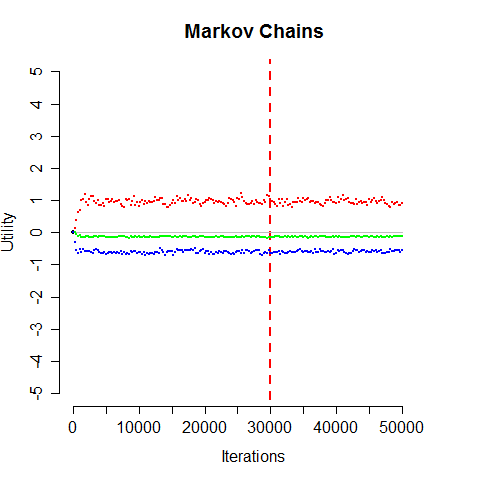
\includegraphics[scale=0.50]{MNL_markovChains2.png}
\label{MarkovChain2}
\end{figure}


\subsection*{Evaluating the output}

As in the first example, current estimates of the markov chains will be plotted to the screen - see figure \ref{MarkovChain2}. In this model, these represent the means of the underlying normals for the random parameters.

There are more output files for this model. RSGHB comes with some basic tools for plotting the contents of these files.

The \emph{.log} file contains some statistics that can be used to understand if model convergence has been reached. Because this model includes random coefficients, the log file now contains the average variance and parameter root mean square (RMS) at each iteration - see figure \ref{logfile2}. 

\begin{figure}
\caption{Plotting of the Log file}
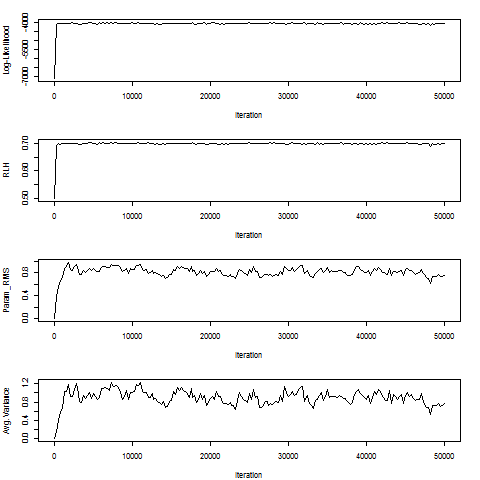
\includegraphics[scale=0.50]{MNL_logPlot2.png}
\label{logfile2}
\end{figure}

The \emph{\_A} file contain the sample-level means of the underlying normal at each iteration.

\begin{Schunk}
\begin{Sinput}
> data(Example2_A)
> head(Example2_A)
\end{Sinput}
\begin{Soutput}
  iteration      ASC1      BTime      BCost
1         1 0.9502366 -0.1249110 -0.5975124
2         2 0.9192204 -0.1345303 -0.6016621
3         3 0.9334093 -0.1275589 -0.5894570
4         4 0.9543322 -0.1385718 -0.5932009
5         5 0.9487994 -0.1187152 -0.5894714
6         6 0.9398888 -0.1178337 -0.5912138
\end{Soutput}
\begin{Sinput}
> 
\end{Sinput}
\end{Schunk}

The \emph{\_B} file contains the average across iterations of the individual level draws for the underlying normals for the random parameters. The \emph{\_Bsd} file provides the standard deviations of those individual draws.

\begin{Schunk}
\begin{Sinput}
> data(Example2_B)
> head(Example2_B)
\end{Sinput}
\begin{Soutput}
  Respondent      ASC1       BTime      BCost
1       8738 1.2065722 -0.01700429 -0.6706683
2       8740 1.1856822 -0.01574887 -0.5232470
3       8741 0.7790173 -0.57719452 -0.4940480
4       8742 1.1593141 -0.27220298 -0.6376389
5       8744 0.5109336 -0.02024900 -0.5083203
6       8745 1.0067985 -0.29565492 -0.5574964
\end{Soutput}
\begin{Sinput}
> data(Example2_Bsd)
> head(Example2_Bsd)
\end{Sinput}
\begin{Soutput}
  Respondent      ASC1     BTime     BCost
1       8738 0.6500682 0.1615823 0.4068272
2       8740 0.6821484 0.1692862 0.4069139
3       8741 0.6917361 0.2080046 0.4230185
4       8742 0.6380699 0.1567093 0.4001571
5       8744 0.7008824 0.1650231 0.4296362
6       8745 0.6259956 0.1675564 0.4018320
\end{Soutput}
\begin{Sinput}
> 
\end{Sinput}
\end{Schunk}

The \emph{\_C} file contains the average across iterations of the individual level draws for the random parameters including the appropriate transformations. The \emph{\_C} file also contains individual-specific measures of model fit (Root Likelihoods). The \emph{\_Csd} file provides the standard deviations of those individual draws. These two files are equivalent to the conditional distributions from models estimated using Maximum Simulated Likelihood methods.

\begin{Schunk}
\begin{Sinput}
> data(Example2_C)
> head(Example2_C)
\end{Sinput}
\begin{Soutput}
  Respondent       RLH      ASC1       BTime      BCost
1       8738 0.6762416 1.2065722 -0.01700429 -0.6706683
2       8740 0.6325542 1.1856822 -0.01574887 -0.5232470
3       8741 0.8420089 0.7790173 -0.57719452 -0.4940480
4       8742 0.5145232 1.1593141 -0.27220298 -0.6376389
5       8744 0.4780804 0.5109336 -0.02024900 -0.5083203
6       8745 0.4919669 1.0067985 -0.29565492 -0.5574964
\end{Soutput}
\begin{Sinput}
> data(Example2_Csd)
> head(Example2_Csd)
\end{Sinput}
\begin{Soutput}
  Respondent      ASC1     BTime     BCost
1       8738 0.6500682 0.1615823 0.4068272
2       8740 0.6821484 0.1692862 0.4069139
3       8741 0.6917361 0.2080046 0.4230185
4       8742 0.6380699 0.1567093 0.4001571
5       8744 0.7008824 0.1650231 0.4296362
6       8745 0.6259956 0.1675564 0.4018320
\end{Soutput}
\begin{Sinput}
> 
\end{Sinput}
\end{Schunk}


The \emph{\_D} file contains a row-based representation of the sample covariance for each iteration. Note the use below of the xpnd function to convert to a matrix representation of the sample covariance.

\begin{Schunk}
\begin{Sinput}
> data(Example2_D)
> head(Example2_D)
\end{Sinput}
\begin{Soutput}
  iteration      ASC1  ASC1xBTime ASC1xBCost        BTime BTimexBCost     BCost
1         1 0.1995635 -0.02084866 0.06611205 -0.012268437  0.03470861 0.1829551
2         2 0.2068453 -0.02099142 0.06574671 -0.005313839  0.03062937 0.1854261
3         3 0.2206137 -0.01672801 0.06778255 -0.000827184  0.03580280 0.1872543
4         4 0.2135790 -0.02085852 0.06905407  0.005535069  0.03119758 0.1801005
5         5 0.2376300 -0.01937409 0.06593123 -0.005413533  0.02932449 0.1752125
6         6 0.2234180 -0.02707077 0.07340550 -0.012843845  0.03041234 0.1790798
\end{Soutput}
\begin{Sinput}
> # building the covariance matrix
> 
> covMat <- xpnd(colMeans(Example2_D[-1]))
> rownames(covMat) <- c("ASC1","BTime","BCost")
> colnames(covMat) <- c("ASC1","BTime","BCost")
> covMat
\end{Sinput}
\begin{Soutput}
             ASC1       BTime       BCost
ASC1   0.44636341 -0.06659140 -0.05475239
BTime -0.06659140  0.07915122  0.03122776
BCost -0.05475239  0.03122776  0.17247616
\end{Soutput}
\end{Schunk}

\section*{RSGHB Control Parameters}

Here is a list of the user-specified control parameters.


\begin{description}

\item[gVarNamesNormal] - A vector of charater-based names for the random parameters. \\
Default: NULL

\item[gVarNamesFixed] - A vector of character-based names for the fixed parameters.\\
Default: NULL

\item[gDIST] - A vector of integers (1-5) which indicate which type of distribution should be applied to the random coefficients - 1 = Normal, 2 = Postive Log-Normal, 3 = Negative Log-Normal, 4 = Censored Normal, 5 = Johnson SB. There should be an element for each name in gVarNamesNormal. \\ Default: NULL

\item[FC] - A vector of starting values for the fixed coefficients. There should be an element for each name in gVarNamesFixed.\\ 
Default: NULL

\item[svN] - A vector of starting values for the means of the underlying normals for the random parameters. There should be an element for each name in gVarNamesNormal.\\ Default: NULL

\item[gNCREP] - Number of burn-in iterations to use prior to convergence.\\ 
Default: 100000

\item[gNEREP] - Number of iterations to keep for averaging after convergence has been reached.\\ Default: 100000

\item[gNSKIP] - Number of iterations in between retaining draws for averaging.\\ 
Default: 1

\item[gINFOSKIP] - Number of iterations in between printing/saving information about the iteration process.
\\ Default: 250

\item[modelname] - The model name which is used for creating output files. 
\\ Default: paste("HBModel",round(runif(1)*10000000,0),sep=""))

\item[gSIGDIG] - The number of significant digits for reporting purposes.\\ 
Default: 10

\item[priorVariance] - The amount of prior variance assumed.\\ 
Default: 2.0

\item[degreesOfFreedom] - Additional degrees of freedom for the prior covariance matrix (not including the number of parameters.\\ 
Default: 5

\item[rho] - The initial proportionality fraction for the jumping distribution for the Metropolis-Hastings algorithm for the random parameters. This fraction is adjusted by the program after each iteration to attain an acceptance rate of about 0.3.\\ 
Default: 0.1

\item[rhoF] - The proportionality fraction for the jumping distribution for the Metropolis-Hastings algorithm for the fixed parameters. Unlike rho, this value is not adjusted as the markov chain proceeds. \\
Default: 0.0001

\item[gFULLCV] - A number that indicates if a full or independent covariance structure should be used for the random parameters. A value of 1 indicated full and 0 for an independent structure.\\ Default: 1

\item[gMINCOEF] - A vector of minimums for the Johnson SB distributions. If Johnson SB is used, each random parameter needs an element but only the elements that correspond to a 5 in gDIST are used. \\ 
Default: 0

\item[gMAXCOEF] - Like gMINCOEF but for the maximum of the Johnson SB distribution. 
\\ Default: 0

\item[gStoreDraws] - A boolean value to store the draws for the individual level coefficients. \\ Default: F

\item[gSeed] - The random seed.\\ 
Default: 0

\item[constraintsNorm] - This is a list of monotonic constraints to be applied during estimation. The structure of the constraints is c(param1number - inequality - param2number). For constraints relative to 0, use 0 instead of the param2number. For the inequality, use 1 for < and 2 for >. Example \begin{verbatim}constraintsNorm <- list(c(5,1,0),c(6,1,5),c(7,1,6),c(8,1,7))\end{verbatim} would constrain the 5th parameter < 0, the 6th parameter < 5th parameter, the 7th parameter < the 6th parameter, etc. \\ Default: NULL

\item[nodiagnostics] - If set to TRUE, the diagnostic report will not be reported to the screen with a prompt to continue. This makes batch processing easier to implement.\\ 
Default: FALSE

\end{description}     


\end{document}
